%%%%%%%%%%%%%%%%%%%%%%%%%%%%%%%%%%%%%%%%%
% Short Sectioned Assignment LaTeX Template Version 1.0 (5/5/12)
% This template has been downloaded from: http://www.LaTeXTemplates.com
% Original author:  Frits Wenneker (http://www.howtotex.com)
% License: CC BY-NC-SA 3.0 (http://creativecommons.org/licenses/by-nc-sa/3.0/)
%%%%%%%%%%%%%%%%%%%%%%%%%%%%%%%%%%%%%%%%%

%----------------------------------------------------------------------------------------
%	PACKAGES AND OTHER DOCUMENT CONFIGURATIONS
%----------------------------------------------------------------------------------------

\documentclass[paper=a4, fontsize=11pt]{scrartcl} % A4 paper and 11pt font size

% ---- Entrada y salida de texto -----

\usepackage[T1]{fontenc} % Use 8-bit encoding that has 256 glyphs
\usepackage[utf8]{inputenc}
%\usepackage{fourier} % Use the Adobe Utopia font for the document - comment this line to return to the LaTeX default

% ---- Idioma --------

\usepackage[spanish, es-tabla]{babel} % Selecciona el español para palabras introducidas automáticamente, p.ej. "septiembre" en la fecha y especifica que se use la palabra Tabla en vez de Cuadro

% ---- Otros paquetes ----

\usepackage{url} % ,href} %para incluir URLs e hipervínculos dentro del texto (aunque hay que instalar href)
\usepackage{amsmath,amsfonts,amsthm} % Math packages
%\usepackage{graphics,graphicx, floatrow} %para incluir imágenes y notas en las imágenes
\usepackage{graphics,graphicx, float, subfig} %para incluir imágenes y colocarlas

% Para hacer tablas comlejas
%\usepackage{multirow}
%\usepackage{threeparttable}

%\usepackage{sectsty} % Allows customizing section commands
%\allsectionsfont{\centering \normalfont\scshape} % Make all sections centered, the default font and small caps

\usepackage{fancyhdr} % Custom headers and footers
\pagestyle{fancyplain} % Makes all pages in the document conform to the custom headers and footers
\usepackage{eurosym} % Para poder añadir el símbolo del euro
\fancyhead{} % No page header - if you want one, create it in the same way as the footers below
\fancyfoot[L]{} % Empty left footer
\fancyfoot[C]{} % Empty center footer
\fancyfoot[R]{\thepage} % Page numbering for right footer
\renewcommand{\headrulewidth}{0pt} % Remove header underlines
\renewcommand{\footrulewidth}{0pt} % Remove footer underlines
\setlength{\headheight}{13.6pt} % Customize the height of the header

\numberwithin{equation}{section} % Number equations within sections (i.e. 1.1, 1.2, 2.1, 2.2 instead of 1, 2, 3, 4)
\numberwithin{figure}{section} % Number figures within sections (i.e. 1.1, 1.2, 2.1, 2.2 instead of 1, 2, 3, 4)
\numberwithin{table}{section} % Number tables within sections (i.e. 1.1, 1.2, 2.1, 2.2 instead of 1, 2, 3, 4)

\setlength\parindent{0pt} % Removes all indentation from paragraphs - comment this line for an assignment with lots of text

\newcommand{\horrule}[1]{\rule{\linewidth}{#1}} % Create horizontal rule command with 1 argument of height
  % Configuración del documento
\usepackage{listings}
\usepackage{color}
\usepackage{tabularx}
\usepackage{graphicx}
\usepackage{array}
\usepackage{hyperref}
\usepackage{url} % ,href} %para incluir URLs e hipervínculos dentro del texto (aunque hay que instalar href)

%----------------------------------------------------------------------------------------
%	TÍTULO Y DATOS DE LOS ALUMNOS
%----------------------------------------------------------------------------------------

\title{	
	\normalfont \normalsize 
	\textsc{\textbf{Inteligencia de Negocio (2019-2020)} \\ Doble grado en Informática y Matemáticas \\ Universidad de Granada} \\ [25pt] 
	\horrule{0.5pt} \\[0.4cm]
	\huge Práctica 3: Competición en DrivenData \\ 
	\horrule{2pt} \\[0.5cm] 
}

\author{Alberto Jesús Durán López \\
		DNI: 54142189-M \\
		Email: albduranlopez@correo.ugr.es \\
		Grupo Prácticas: Martes} 
\date{\normalsize\today}

%----------------------------------------------------------------------------------------
% DOCUMENTO
%----------------------------------------------------------------------------------------

\definecolor{mygreen}{rgb}{0,0.6,0}
\definecolor{mygray}{rgb}{0.5,0.5,0.5}
\definecolor{mymauve}{rgb}{0.58,0,0.82}
\definecolor{mygray2}{rgb}{0.93,0.93,0.93}

\lstset{ 
	backgroundcolor=\color{mygray2},   % choose the background color; you must add \usepackage{color} or \usepackage{xcolor}; should come as last argument
	basicstyle=\footnotesize,        % the size of the fonts that are used for the code
	breakatwhitespace=false,         % sets if automatic breaks should only happen at whitespace
	breaklines=true,                 % sets automatic line breaking
	captionpos=b,                    % sets the caption-position to bottom
	commentstyle=\color{mygreen},    % comment style
	deletekeywords={...},            % if you want to delete keywords from the given language
	escapeinside={\%*}{*)},          % if you want to add LaTeX within your code
	extendedchars=true,              % lets you use non-ASCII characters; for 8-bits encodings only, does not work with UTF-8
	firstnumber=-1   ,                % start line enumeration with line 1000
	frame=Simple,	                   % adds a frame around the code
	keepspaces=true,                 % keeps spaces in text, useful for keeping indentation of code (possibly needs columns=flexible)
	keywordstyle=\color{blue},       % keyword style
	language={Python}  ,                 % the language of the code
	morekeywords={*,...},            % if you want to add more keywords to the set
	numbers=left,                    % where to put the line-numbers; possible values are (none, left, right)
	numbersep=5pt,                   % how far the line-numbers are from the code
	numberstyle=\tiny\color{mygray}, % the style that is used for the line-numbers
	rulecolor=\color{black},         % if not set, the frame-color may be changed on line-breaks within not-black text (e.g. comments (green here))
	showspaces=false,                % show spaces everywhere adding particular underscores; it overrides 'showstringspaces'
	showstringspaces=false,          % underline spaces within strings only
	showtabs=false,                  % show tabs within strings adding particular underscores
	stepnumber=2,                    % the step between two line-numbers. If it's 1, each line will be numbered
	stringstyle=\color{mymauve},     % string literal style
	tabsize=2,	                   % sets default tabsize to 2 spaces
	title=\lstname                   % show the filename of files included with \lstinputlisting; also try caption instead of title
}



\begin{document}
	\maketitle       % título
	\newpage 
	
	\begin{figure}[H]
		\centering
		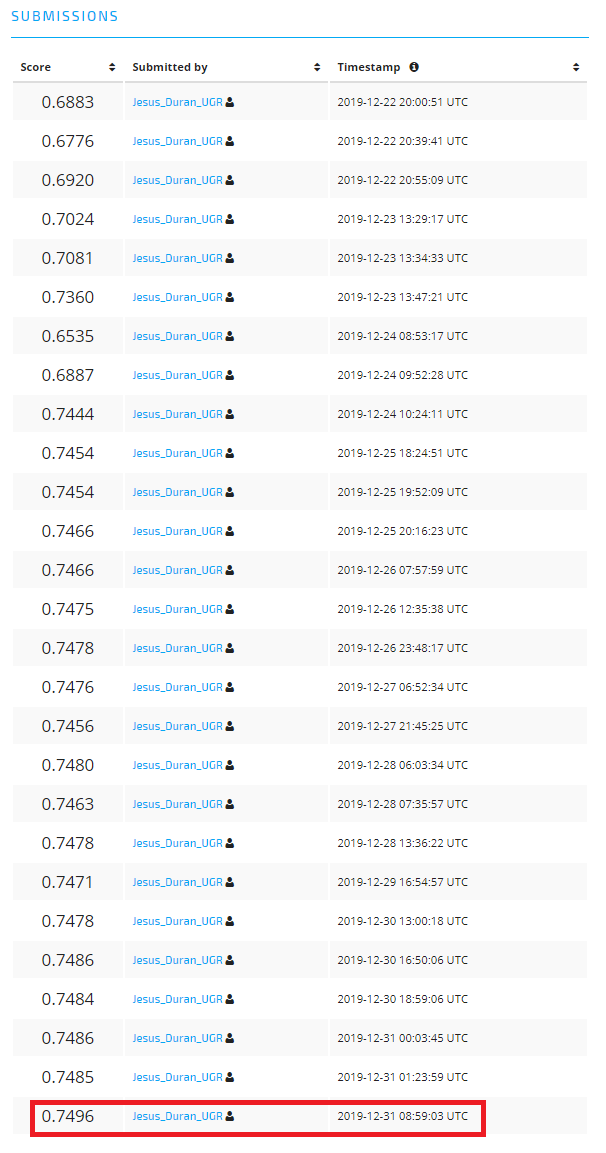
\includegraphics[width=0.81\textwidth]{img/subs.png}
		\caption{Submissions}
	\end{figure}
	
	\tableofcontents % índice
	\newpage
	
	
	
	\section{Introducción}
	
		\hspace{1.5cm} En esta práctica usaremos métodos avanzados para aprendizaje supervisado en clasificación y participaremos en una competición real de DrivenData (\url{https://www.drivendata.org/}
	
	El problema a resolver es \textit{Richter's Predictor: Modeling Earthquake Damaga}, disponible en \url{https://www.drivendata.org/competitions/57/nepal-earthquake/} \\
	
	El objetivo es el de predecir el nivel de daño a los edificios causados por un terremoto, \texttt{Gorkha}, en 2015 en Nepal.  Se usarán los datos proporcionados por la Oficina Central de Estadística y se trabajará especialmente con el conjunto de datos de entrenamiento.
	 
	
	A partir de un preprocesado de los datos junto a diferentes pruebas de algoritmos, se intentará mejorar nuestro modelo. \\
	
	Para realizar una primera primera ejecución contamos únicamente con la descripción de las características, disponible en \url{https://www.drivendata.org/competitions/57/nepal-earthquake/page/136/} y con un ranking de las primeras 50 posiciones, desconociendo el procedimiento usado para cada uno de ellos.
	
	
	
	
	
	
	
	

\section{Estudio del DataSet}

\hspace{1.5cm} El conjunto de datos de entrenamiento consta de 260.601 instancias y 39 atributos categóricos, binarios y enteros. 

 Se predecirá la variable \texttt{damage\_grade} la cual representa la cantidad de daño que se ha producido al edificio. Esta variable puede tomar los valores 1, 2 y 3, que representan un daño bajo, una cantidad media de daño y una destrucción casi completa, respectivamente. \\


Estudiando las variables de los datos proporcionados y, con la ayuda de una pequeña función en python, observamos que no presentan valores perdidos, por lo que no es necesario imputar dichos valores. \\


\begin{lstlisting}[frame=single]
print("Valores perdidos:")
print(data_training.isnull().sum())
data_training.isnull().sum().plot.bar()
plt.show()
\end{lstlisting}
El gráfico correspondiente al código anterior muestra que todas las variables contienen un total de 0 valores perdidos. \\


Sin embargo, esto no supondría ningún problema usando la clase \textit{Imputer} que nos proporciona sklearn. Se podría realizar la siguiente función para imputar dichos valores por la estrategia seleccionada, es decir, \textit{mean}, \textit{median} o \textit{most\_frequent}. \\
Mostramos a continuación el fragmento de código referido: \\

	\begin{lstlisting}[frame=single]
def ImputarStrategy(strat):
		imp = Imputer(missing_values='NaN', strategy=strat)
		imp = imp.fit(X)
		X_train_imp = imp.transform(X)
		imp = imp.fit(X_tst)
		X_tst_imp = imp.transform(X_tst)
	
		return X_tst_imp, X_train_imp\end{lstlisting}	
		

Por otro lado, mostramos las clases con la ayuda del siguiente diagrama de barras:


\begin{figure}[H]
	\centering
	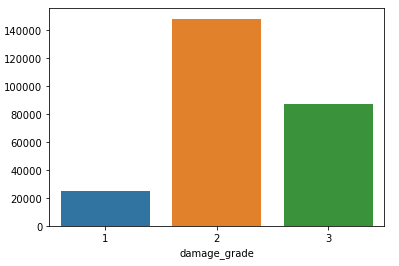
\includegraphics[width=0.65\textwidth]{img/grade.png}
	\caption{Clases}
\end{figure}


Podemos observar (en color naranja), que la clase predominante es la número 2 (con más de 140.000 instancias), seguida de la clase 3 y dejando con apenas 20.000 instancias la clase 1. El desbalanceo de clases supone un grave problema en el aprendizaje automático y obtener un muestreo equilibrado de las clases supondría una mejora en muchos escenarios. \hfill

Dejaremos el problema del desbalanceo de clases para secciones posteriores, donde se explicará con profundidad como hacer frente a dicho problema.

\newpage
Por último, procedemos a mostrar un heatmap o mapa de calor donde se muestra la correlación de las variables:

\begin{figure}[H]
	\centering
	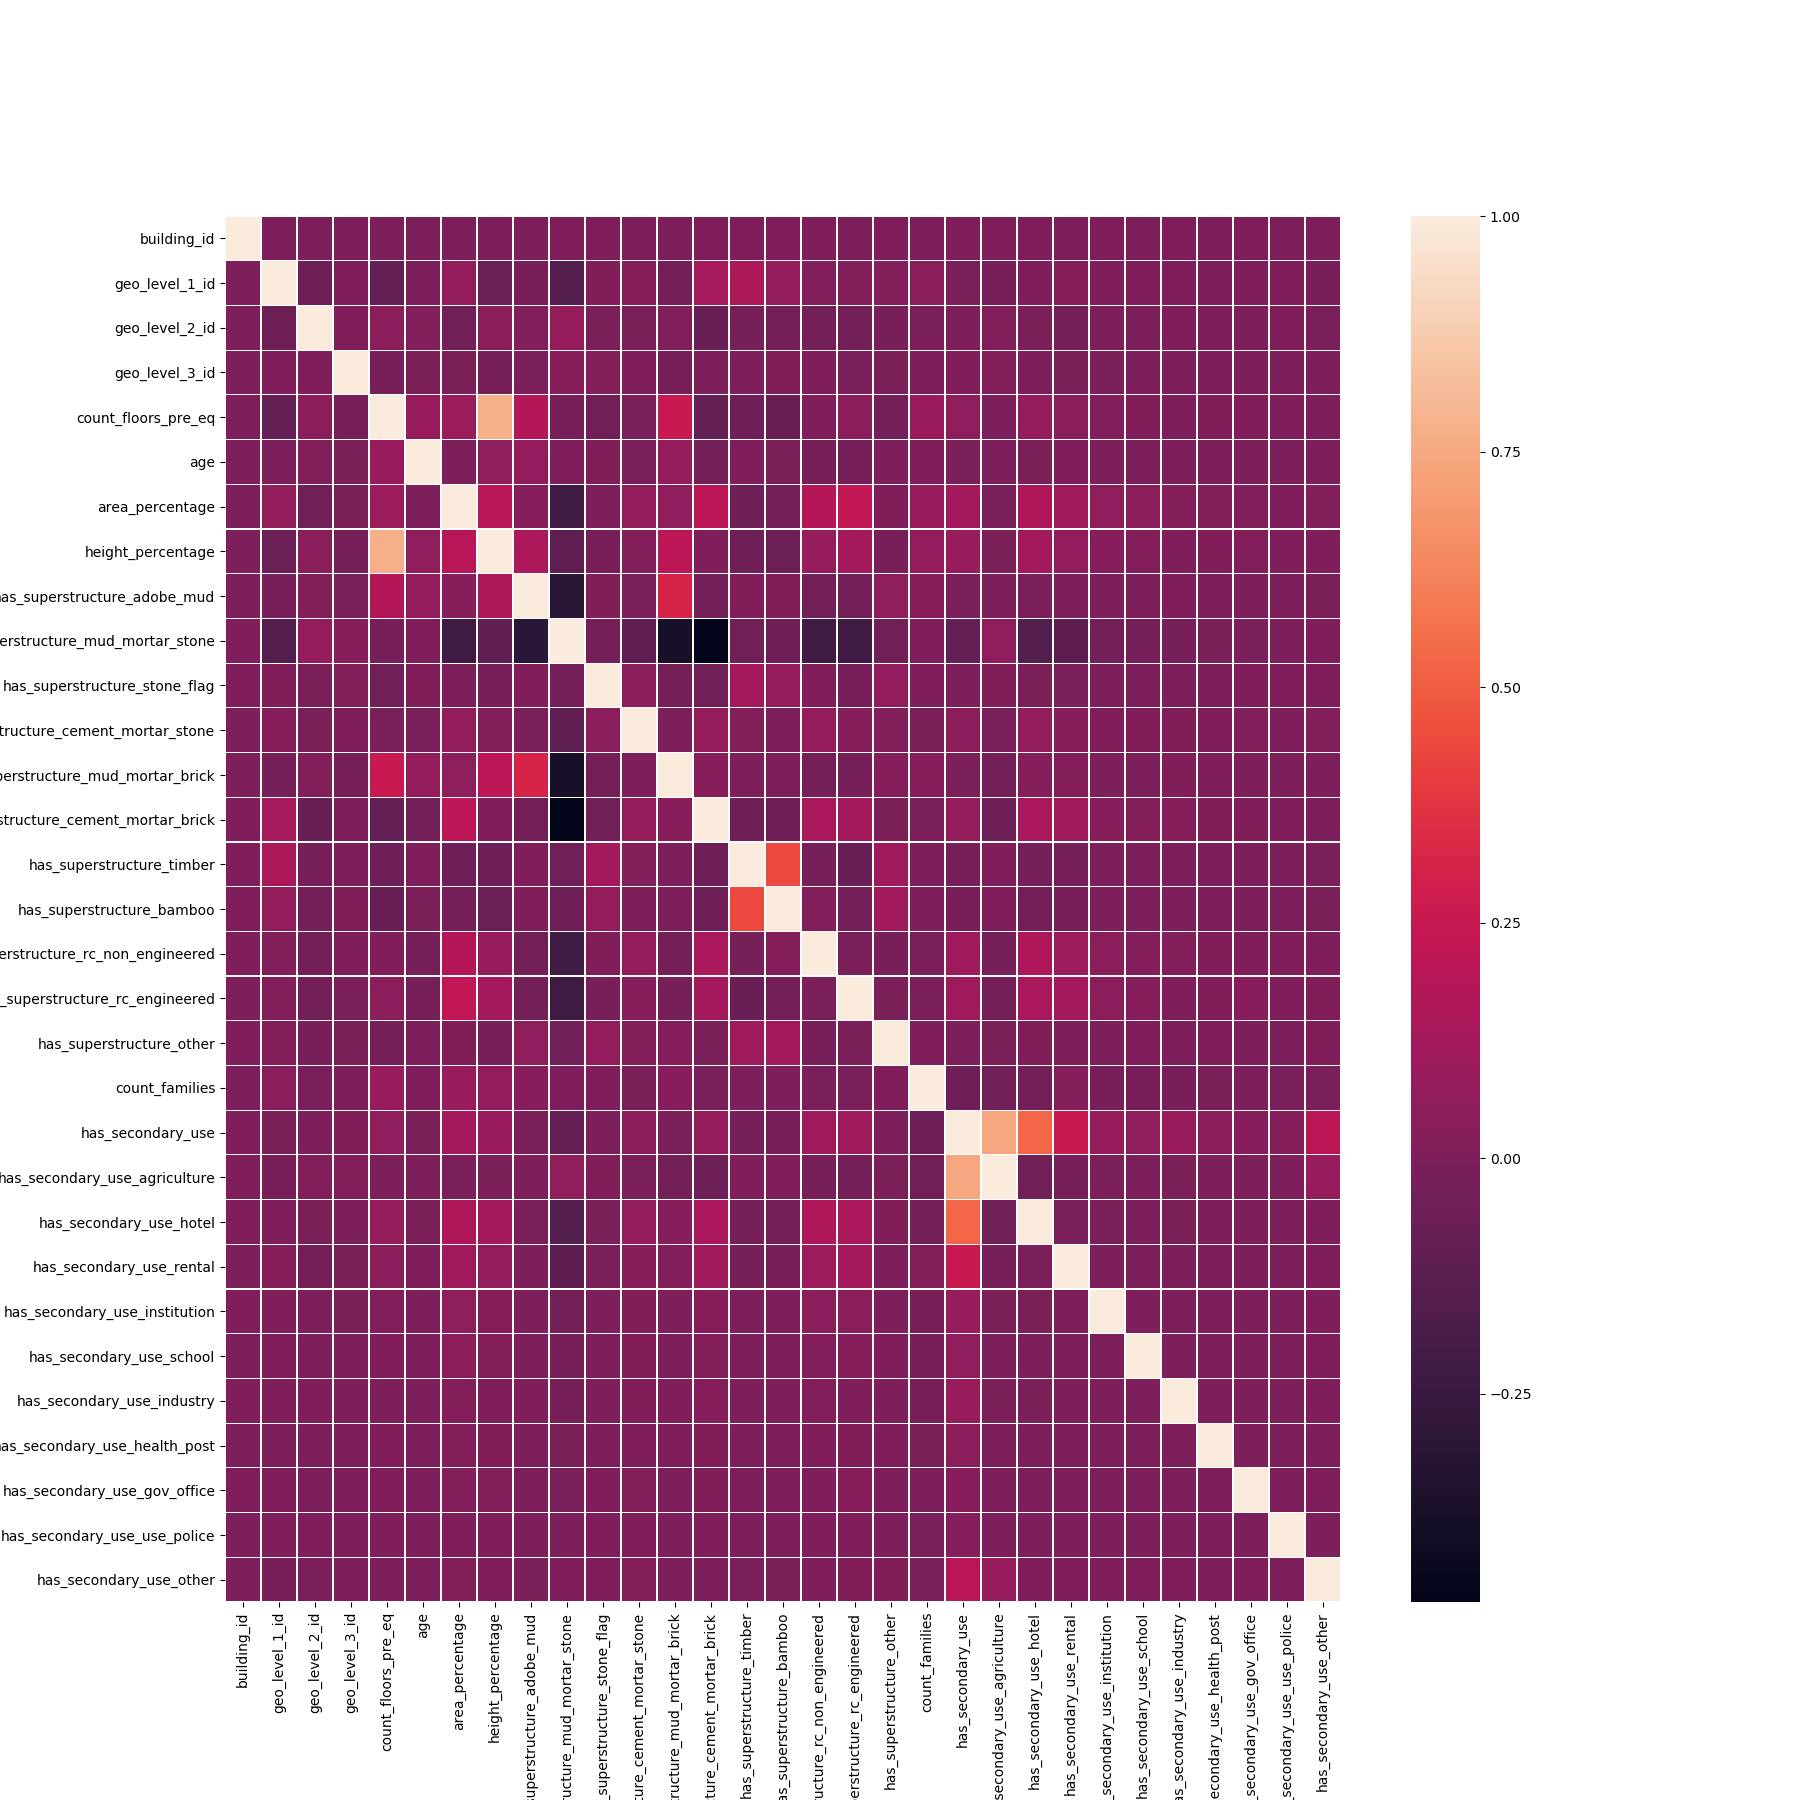
\includegraphics[width=0.96\textwidth]{img/corr.png}
\end{figure}

En el heatmap anterior los colores más claros representan una correlación mayor respecto a los colores más oscuros. 


Se ha eliminado la variable \texttt{building\_id}, que contiene un identificador único para cada edificio y no aporta nada al conjunto del dataset. Por otro lado, en nuestro dataset existen muchos atributos del tipo \textit{has\_secondary\_use}, variable que está relacionada con el resto de variables que se llaman de forma similar: \textit{has\_secondary\_use...}.


Tras realizar algunos intentos de eliminar alguna otra variable (usando por ejemplo la herramienta \textit{Boruta}), se ha comprobado que no hay apenas ruido en la base de datos y que en resumen, todas las variables 'aportan' algo por lo que los intentos de eliminar las variables menos significativas han sido en vano.


\section{Preprocesado}

\hspace{1.5cm} Realizamos distintos tipos de preprocesado a nuestros datos, explicaremos cada uno de ellos detalladamente:

\subsection{Variables numéricas y categóricas}
\begin{itemize}
	\item \textbf{Preprocesado Inicial}: Se trata del preprocesado que venía por defecto, proporcionado por el profesor. Transforma variables numéricas a categóricas. Sin embargo, los algoritmos no se veían potenciados, por lo que procedemos a realizar otro tipo de preprocesado a las variables categóricas.
	
	
	\item \textbf{Biyección con números naturales -  \texttt{[Preprocesado1]}}: Establecemos una biyección con los números naturales para transformar las variables categóricas a numéricas. A cada letra del abecedario le hacemos corresponder su número natural asociado, es decir:
	
	a $\rightarrow$ 1 , b $\rightarrow$ 2 , c $\rightarrow$ 3 , ... , z $\rightarrow$ 27
	
	Se realiza tal y como se muestra a continuación:

	\begin{lstlisting}[frame=single]
biyeccion = {'a':1, 'b':2, 'c':3, 'd':4, 'e':5, 'f':6, 'g':7, 
	'h':8, 'i':9, 'j':10, 'k':11, 'l':12, 'm':13, 'n':14, 
	'/n':15,'o':16, 'p':17, 'q':18, 'r':19, 's':20,'t':21, 
	'u':22, 'v':23, 'w':24, 'x':25, 'y':26, 'z':27}
	
preprocesado1 = {"roof_type": biyeccion,
	"land_surface_condition": biyeccion,
	"position": biyeccion,
	"other_floor_type": biyeccion,
	"legal_ownership_status": biyeccion,
	"foundation_type": biyeccion,  
	"ground_floor_type": biyeccion,
	"plan_configuration": biyeccion,
}
	\end{lstlisting}
	
	
	\item \textbf{Restringir dominio variables  - \texttt{[Preprocesado2]}}:
	Observando el archivo .csv proporcionado para realizar la práctica, podemos comprobar que las variables numéricas toman pocos valores. Es por esto por lo que se podría realizar una modificación a la biyección anterior y restringir el dominio que toman las variables.
	Ordenamos por orden alfabético los valores que pueden tomar las variables categóricas y le asignamos los números naturales, empezando por el 1 y de forma ascendente, tal y como mostramos a continuación:
	
	\begin{lstlisting}[frame=single]
	
preprocesado2 = {"roof_type": {'n': 1, 'q': 2, 'x': 3},
	"land_surface_condition": {'n': 1, 'o': 2, 't':3},
	"position": {'j': 1, 'o': 2, 's': 3, 't': 4},
	"other_floor_type": {'j': 1, 'q': 2, 's': 3, 'x': 4},
	"legal_ownership_status": {'a':1,'r':2,'v':3,'w':4},         
	"foundation_type":{'h':1,'i':2,'r':3,'u':4,'w':5},               
	"ground_floor_type": {'f':1,'m':2,'v':3,'x':4, 'z':5},
	"plan_configuration": {'a': 1, 'c': 2, 'd': 3, 'f': 4, 
	     'm': 5, 'n': 6, 'o': 7, 'q': 8, 's': 9, 'u': 10}
	}
	\end{lstlisting}
	
	El uso de este preprocesado obtiene prácticamente los mismos resultados que el preprocesado1, no estableciendo una clara mejora.
	
	\item \textbf{Get Dummies - \texttt{[Preprocesado3]}}: Se puede usar este método para convertir variables categóricas en variables numéricas. Con esto, se obtiene la columna categórica y genera de manera automática una lista de números (que pueden ser 1 si contiene la cadena o 0 en caso contrario), cada uno correspondiente a una categoría particular de la variable. \\ Sin embargo, aplicamos getDummies al conjunto de variables total, tal y como se muestra a continuación:
	
	\begin{lstlisting}[frame=single]
data_training = pd.get_dummies(data_training)
data_test = pd.get_dummies(data_test)
	\end{lstlisting}

\end{itemize}


\subsection{Balanceo de clases}
Otro problema de los datos proporcionados es que las clases están desbalanceadas como hemos comentado anteriormente, lo que se ve reflejado en un peor resultado, cosa que se podría evitar balanceando las clases \\ 
Principalmente existen estas dos formas:

\begin{itemize}
	\item \textbf{Algoritmos preparados para clases desbalanceadas}: Como bien se indica, existen algoritmos preparados con un parámetro para tratar el problema del desbalanceo de clases. 
	Cuando se incluye este parámetro, el modelo por lo general actúa de forma automática aplicando una métrica por defecto, como es el caso de \texttt{is\_unbalance} de \textit{LightGBM}.
	
	Por otro lado, existen algoritmos como el propio \textit{LightGBM} o \textit{Random Forest} donde podemos ajustar los pesos de las clases de forma automática o manual con el parámetro \texttt{class\_weight} o \texttt{scale\_pos\_weight}.
	
	\item \textbf{Smote}:  Herramienta muy útil para realizar un oversampling de los datos de forma sencilla. Es necesario instalar el paquete \texttt{smote\_variants}.
	
	Existen bastantes variantes disponibles en : \url{https://github.com/gykovacs/smote_variants}, además, se incluye una descripción y ejemplos de cada uno, mostrando incluso un ranking con los mejores resultados:
	
	\begin{figure}[H]
		\centering
		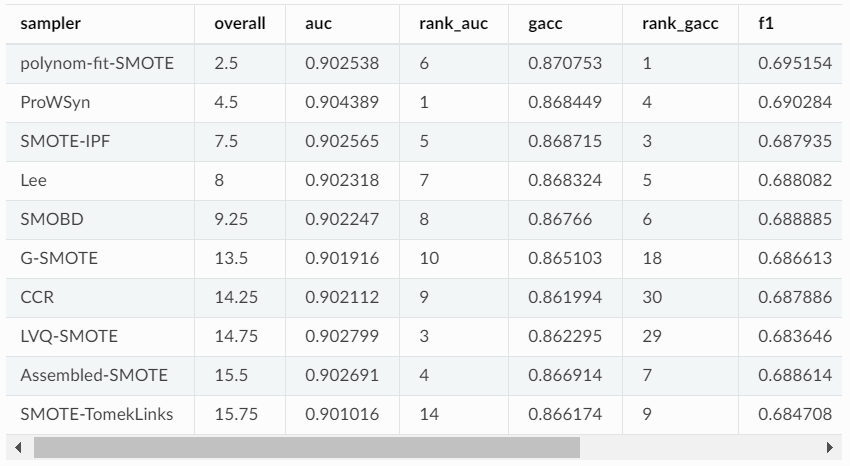
\includegraphics[width=1\textwidth]{img/smoter.png}
		\caption{Ranking mejores Smote}
	\end{figure}

	
	Como norma general, equilibrar las clases realizando un oversampling no es recomendable, lo adecuado y óptimo sería obtener un equilibrio en las clases, realizando un undersampling de la clase superior y un oversampling de la inferior, obteniendo así el número de instancias de la clase intermedia.
	
	Sin embargo, debido a que nuestro dataset no presenta outliers ni ruido, en las últimas submissions se ha realizado un oversampling a la clase superior y se han obtenido resultado bastante prometedores.
	
	En nuestro caso probamos dos variantes, \textit{distance\_SMOTE} \textit{Polynom-fit-SMOTE} que explicaremos a continuación:
	
	\newpage
	
	\begin{itemize}
		\item \textbf{Distance SMOTE}
		\begin{lstlisting}[frame=single]
oversampler= sv.MulticlassOversampling(sv.distance_SMOTE())
		\end{lstlisting}
		
		El número de instancias de las 3 clases queda totalmente balanceado, obteniendo un total de instancias de la clase superior para cada una de ellas. Desde la submission 23 hasta la 26 se hace uso de esta variante. 
		
		
		\begin{figure}[H]
			\centering
			\subfloat[Unbalanced]{
				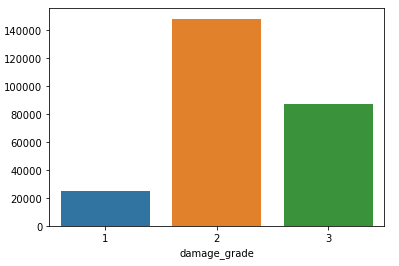
\includegraphics[width=0.55\textwidth]{img/grade.png}}
			\subfloat[Balanced]{
				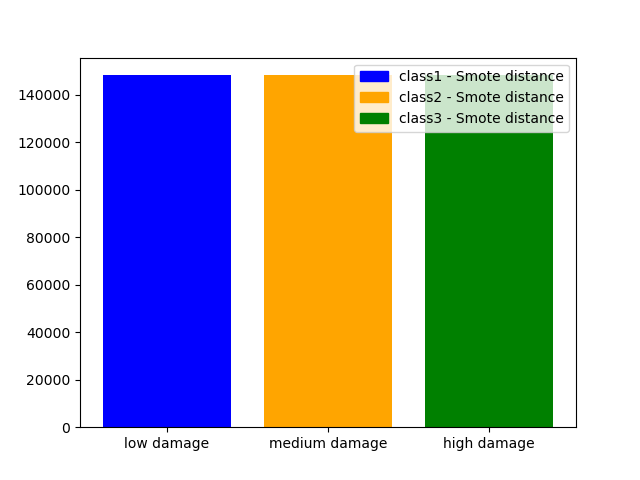
\includegraphics[width=0.55\textwidth]{img/distance.png}}
		\end{figure}
	
	
	La documentación oficial disponible quizás es algo escasa y al incluir el término \textit{distance} pensamos que quizás era necesario normalizar los datos (proceso que no hacemos porque estamos ante un algoritmo basado en árboles). Por esto mismo, preferimos probar otra variante y comprobar si los resultados mejoran. \\
		
		
		\item \textbf{Polynom-fit-SMOTE}: Ocupa el rank1 en la clasificación de los SMOTE que se ha incluído en la página anterior. 

		\begin{lstlisting}[frame=single]
oversampler=sv.MulticlassOversampling(sv.polynom_fit_SMOTE(topology='star')
		\end{lstlisting}
		Como parámetro, incluímos la topología \textit{star}, aunque dicha elección no es única, pudiendo elegir entre otras opciones como \textit{mesh} o \textit{bus}
	
	
	\begin{figure}[H]
		\centering
		\subfloat[Unbalanced]{
			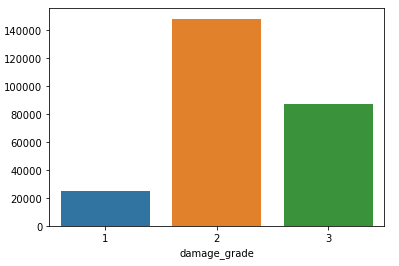
\includegraphics[width=0.55\textwidth]{img/grade.png}}
		\subfloat[Balanced]{
			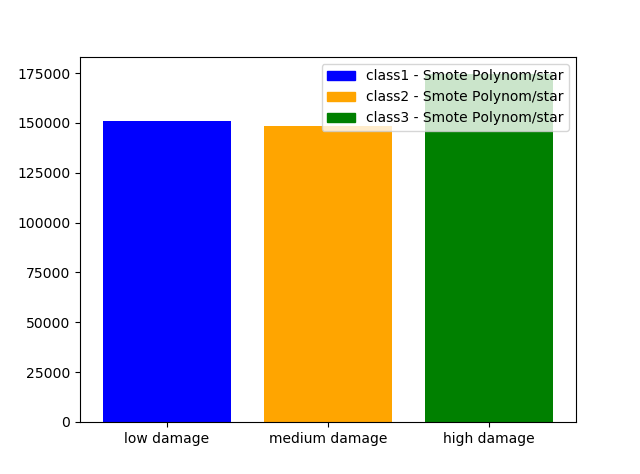
\includegraphics[width=0.55\textwidth]{img/sstar.png}}
		
	\end{figure}

		En este caso, las clases no están completamente balanceadas. La clase 1 y 2 tienen una ligera diferencia, rondando las 140.000 instancias,  mientras que la clase 3 llega incluso a las 175.000 instancias. Aunque pueda parecer extraño, con este ligero desbalanceo se obtienen los mejores resultados de todos.
		
		
		
	
	\end{itemize}
	

	
	
\end{itemize}



	
	
	\section{Algoritmos}
	
		\hspace{1.5cm} En esta sección explicaremos los diferentes algoritmos usados, así como ventajas y desventajas encontradas en el estudio de los modelos. \\
	
	
	
	Antes de adentrarnos en dicho estudio, cabe destacar el  empleo de técnicas como \texttt{GridSearch}, herramienta que ante una serie de parámetros, escoge los mejores para el modelo. Principalmente se eligen de forma exhaustiva cuales son los mejores parámetros para entrenar el modelo, evitando a toda costa el underfitting y el overfitting que se produce en el proceso de entrenamiento.
	
	\newpage
	
	A continuación mostramos un ejemplo realizado de \texttt{GridSearch} en el que calculamos de entre los parámetros indicados, los mejores: \\
	
	\begin{figure}[H]
		\centering
		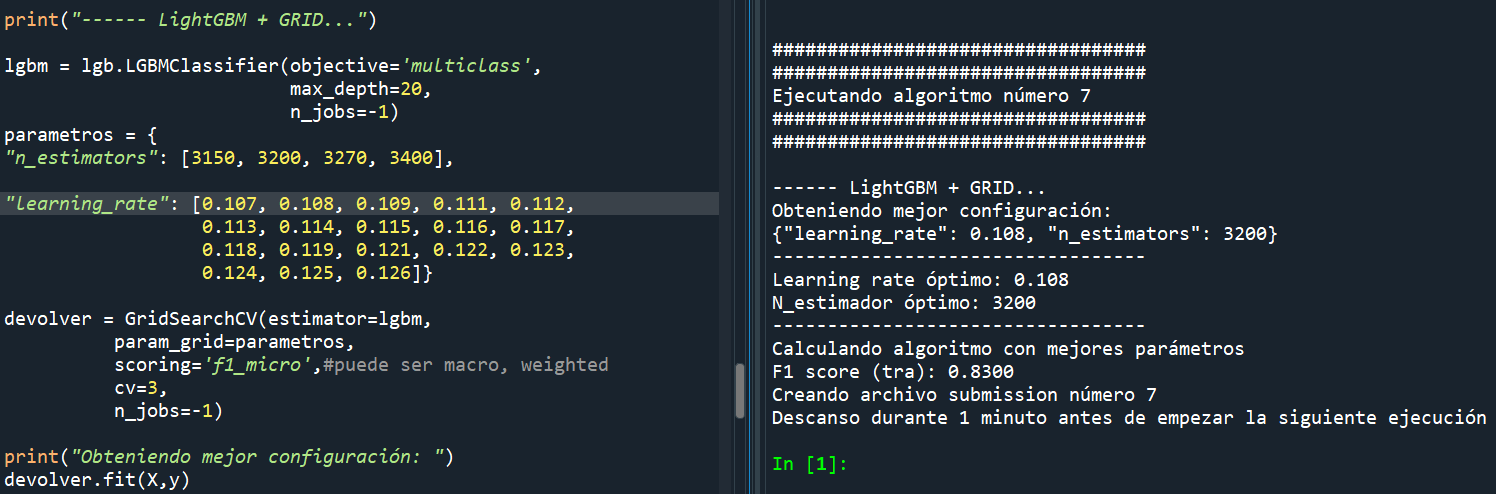
\includegraphics[width=1.1\textwidth]{img/Capturanew.png}
		\caption{Ejecución GridSearchCV}
	\end{figure}

	Otra técnica que se podría haber usado es \texttt{RandomSearch}, útil cuando se desea ahorrar en tiempo y el número de instancias no supone un problema. Se han realizado ejecuciones con grid para ajustar parámetros usuales como \textit{n\_estimators, learning\_rate, max\_depth} y otros menos usuales como \textit{objective, is\_unbalance} o incluso \textit{class\_weight}, para ajustar de forma óptima el peso que le asignamos a cada clase.
	
	
	\begin{itemize}
		
		
		\item \textbf{XGBoost}: Extreme Gradient Boosting. Se trata de una implementación de árboles de decisión con Gradient Boosting diseñada para minimizar la velocidad de ejecución y maximizar el rendimiento.
		
		En nuestras pruebas no obteníamos un score en el training lo suficientemente alto como para subirlo a Drivendata, ya que teníamos únicamente 3 submission al día y no había que arriesgar, además, el tiempo de ejecución era bastante superior al resto por lo que el ajuste de hiperparámetros se complicaba.
		
		
		\item \textbf{LightGBM}: Light Gradient Boosting Machine. Basada en árboles de decisión y paralelización masiva de modelos. Se caracteriza por ser muy eficaz a la hora de ejecutar los modelos.
		
		
		Es el algoritmo que mejor resultados nos ha dado con diferencia. Su eficiencia destacaba por encima del resto, además, hablando en términos de eficacia y bajo los mismos parámetros, era incluso superior a otros modelos, resultando en un gran ahorro de tiempo a la hora de realizar el ajuste de hiperparámetros. 
		
		Algunas de estas ejecuciones se han guardado en el archivo \textbf{RESULTADOS.CSV}, disponible en la carpeta \textbf{Submissions} entregada en la práctica. El resto de resultados de grid se han incluído como comentarios en el código \textit{earthquake.py}.
		
		\newpage
		
		\begin{lstlisting}[frame=single]
lgbm = lgb.LGBMClassifier(objective='multiclassova',
			  									learning_rate=0.108,
								  				n_estimators=3198,
								  				max_depth=20,
											  	random_state=seed,
											  	class_weight={1: 1, 2: 0.8, 3: 0.7})
		\end{lstlisting}
		
		
		En el fragmento de código anterior se muestra un ejemplo de ejecución tras haber realizado un ajuste óptimo de los parámetros, correspondiente a la submission 17.
		
		\item \textbf{Random Forest}: Se trata de un meta estimador que ajusta un número de árboles de decisión en muestras del dataset para después realizar un promedio y mejorar la precisión a la vez que se controla el over-fitting.  
		
		Es un método versátil de aprendizaje automático capaz de realizar tanto tareas de regresión como de clasificación. Está incluído en la biblioteca de \textit{scikit-learn} y se construye de la siguiente forma: \\
		
		\begin{lstlisting}[frame=single]
rf = RandomForestClassifier(n_estimators=500, 
												    learning_rate=0.1, max_depth=20, 	
												    min_samples_split=2,
												    random_state=seed,
												    class_weight='balanced')	
		\end{lstlisting}
		
		
		
		Los principales parámetros de este clasificador son \texttt{n\_estimators} y \texttt{learning\_rate}, teniendo que un aumento del número de estimadores resulta en un tiempo mayor de ejecución pero quizás no una mayor precisión. Por otro lado, un mayor \texttt{learning\_rate} se ve reflejado en un modelo que reacciona más rápido ante los datos que van llegando pero  propenso a un overfitting superior. En el caso de este algoritmo, era bastante complicado establecer un \textit{learning\_rate} óptimo, obteniendo en la mayoría de ejecuciones un resultado con bastante overfitting en el training.
		
				
		\item \textbf{CatBoost}: Algoritmo de aprendizaje automático basado en potenciación del gradiente \textit{'Gradient Boosting'}. El nombre de CatBoost proviene de la unión de Category y Boosting, donde el primer término hace referencia al hecho de que la librería funciona perfectamente con variables categóricas. 
		
		
		\newpage
		\begin{lstlisting}[frame=single]
cbc= CatBoostClassifier(learning_rate=0.1,
												n_estimators=550,
												loss_function='MultiClass',
												eval_metric='TotalF1',
												od_pval=0.001,
												od_type='IncToDec',
												random_seed=54142189,
												bootstrap_type='MVS', #Probar Bayesian
												best_model_min_trees=250,
												max_depth=12)
		\end{lstlisting} 
		
		Con la configuración mostrada anteriormente, se llegó a obtener un F1-Score de 0.7360 en la submission 6, sin embargo, el tiempo de ejecución era bastante superior al resto y se descartó por las mismas razones que \texttt{XGBoost}
		
		\item \textbf{BaggingClassifier}: \textbf{B}ootstrap \textbf{Agg}regat\textbf{ing}. Técnica que entrena diferentes muestras del dataset original (con la misma cardinalidad) usando combinaciones con repetición, combinando todas ellas y obteniendo una predicción final en la cual la varianza se ha reducido. 
		
		Ha resultado ser una técnica esencial en el desarrollo de nuestro modelo final, mejorando por varias centésimas nuestro Score final. Para dicho clasificador, se han realizado variaciones y ejecuciones con \texttt{GridSearch} en el número de estimadores y en el parámetro booleano \textit{Bootstrap}, que indica si las muestras se extraen con reemplazamiento (True), o en caso contrario, sin él (False). Tras probar y ejecutar durante varios días, no se obtuvo una configuración adecuada, dejando todo azar. \\
		
		
		
		\begin{lstlisting}[frame=single]
lgbm = lgb.LGBMClassifier(...)
		
clf=BaggingClassifier(
			base_estimator=lgbm,
			n_estimators=15,
			bootstrap=True) #A veces se obtiene mejor resultado con False
		\end{lstlisting} 
		
		\hfill
		\hfill
		\item \textbf{VotingClassifier}: Herramienta que requiere el entrenamiento de diversos algoritmos para después unirlos y predecir la salida final.  \\
		Para un resultado óptimo de este clasificador es conveniente el uso y entrenamiento de algoritmos diferentes (basados en árboles, reglas, probabilisticos...etc). \\
		
		\newpage
		 En nuestro caso usamos únicamente \textit{LightGBM} con diferentes parámetros potenciando el resultado final uniendo dos bagging (uno de ellos con Bootstrap=True y otro con esta variable tomando un valor False) y juntándolo en este Voting, tal y como se muestra a continuación: \\
		
		
		\begin{lstlisting}[frame=single]
lgbm1=lgb.LGBMClassifier(learning_rate=0.1, objective='multiclassova',
												 n_estimators=3198, n_jobs=-1,
												 num_leaves=34, max_bin=500,
												 max_depth=22, random_state=seed)

lgbm2=lgb.LGBMClassifier(learning_rate=0.1, objective='multiclassova',
											   n_estimators=3198, n_jobs=-1,
												 num_leaves=34, max_bin=500,
												 max_depth=24, random_state=seed)

clf1 = BaggingClassifier(base_estimator=lgbm1, n_estimators=20,
												 bootstrap=False, random_state=seed)

clf2 = BaggingClassifier(base_estimator=lgbm2, n_estimators=15,
												 bootstrap=False, random_state=seed)

devolver = EnsembleVoteClassifier(clfs=[clf1, clf2],
																	weights=[1, 1], voting='soft')
		\end{lstlisting}
		
		El resultado tras ejecutar este modelo combinado, superando incluso las 5 horas de ejecución, ha sido la combinación perfecta (junto con oversampling de SMOTE). 
		Es el seleccionado para la submission final, obteniendo un F1-Score de 0.7496 y un rank final de 34.
		
		
		\begin{figure}[H]
			\centering
			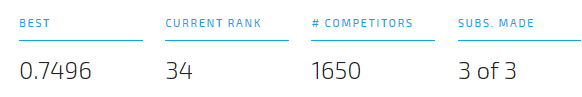
\includegraphics[width=0.8\textwidth]{img/pole1.png}
		\end{figure}
		
		Como nota aclaratoria, \texttt{EnsembleVoteClassifier} tiene un parámetro \textit{voting} que puede tomar valor 'hard' o 'soft'. En el caso de 'hard', el clasificador cuenta el número de instancias más votada y toma dicho valor. Por otro lado, cuando los modelos están mejor entrenados (como es nuestro caso, debido a la gran cantidad de GridSearch que se esconden tras él) es recomendable el uso de 'soft' en el que se indica al clasificador que realice una media de las probabilidades de cada instancia.
		
		\item \textbf{Otros}: Se han usado otros algoritmos como LogisticRegression, pero a la hora de realizar pruebas con sus parámetros no se han obtenido buenos resultados en el training. Esto es sucede porque al no ser algoritmos basados en árboles, necesitan un preprocesado básico de normalización de variables.
	\end{itemize}
	
	
	
	
	
	
	
	
	\section{Resultados}
	
	\hspace{1cm} Mostramos una tabla a modo de resumen de cada una de las subidas realizadas a Drivendata, incluyendo la fecha de subida, el rank tras subir la submission, algoritmo usado, configuración\&preprocesado y tanto el score obtenido en el training como en el test\\
	
	
	% Please add the following required packages to your document preamble:
	% \usepackage{graphicx}
	\begin{table}[H]
		\centering
		\resizebox{1.05\textwidth}{!}{%
			\begin{tabular}{ccccccc}
				\hline
				\textbf{Submission} & \textbf{Date}           & \textbf{Rank} & \textbf{Algorithm}               & \textbf{Score tra} & \textbf{Score tst} & \textbf{Configuration and Preprocessing}                 \\ \hline
				1                   & 22/12/2019-8pm          & 377           & LightGBM/CrossValidation         & 0.7264             & 0.6883             & Configuración y preprocesado inicial                     \\
				2                   & 22/12/2019-9pm          & 377           & XGBoost/Cross Validation         & 0.6886             & 0.6776             & Configuración y preprocesado inicial                     \\
				3                   & 22/12/2019-9pm          & 356           & Random Forest                    & 0.7692             & 0.6920             & Configuración y preprocesado inicial                     \\
				4                   & 23/12/2019-1pm          & 332           & CatBoost                         & 0.7856             & 0.7024             & Configuración y preprocesado inicial                     \\
				5                   & 23/12/2019-2pm          & 316           & Random Forest                    & 0.7659             & 0.7081             & Preprocesado1, 350 estimators                            \\
				6                   & 23/12/2019-2pm          & 180           & CatBoost                         & 0.7903             & 0.7360             & Preprocesado1, 550 estimators                            \\
				7                   & 24/12/2019-9am          & 180           & CatBoost                         & 0.8555             & 0.6535             & Preprocesado inicial, oversampling smote                 \\
				8                   & 24/12/2019-10am         & 180           & Random Forest                    & 0.7548             & 0.6887             & Preprocesado1, asignando pesos(class\_weight)            \\
				9                   & 24/12/2019-10am         & 110           & LightGBM                         & 0.8011             & 0.7444             & Preprocesado2, is\_unbalance, 2000 estimators            \\
				10                  & 25/12/2019-6pm          & 98            & LightGBM/GridSearch              & 0.8272             & 0.7454             & Preprocesado2, is\_unbalance, 2950 estimators            \\
				11                  & 25/12/2019-8pm          & 98            & LightGBM/CrossValidation         & 0.8272             & 0.7454             & Preprocesado2, is\_unbalance, 3198 estimators            \\
				12                  & 25/12/2019-8pm          & 81            & LightGBM/GridSearch              & 0.8299             & 0.7466             & Conf. anterior ajustando con GridSearch                  \\
				13                  & 26/12/2019-8am          & 81            & LightGBM/GridSearch              & 0.8299             & 0.7466             & GridSearch, scale\_pos\_weight=0.5                       \\
				14                  & 26/12/2019-1pm          & 72            & LightGBM/Bagging                 & 0.8213             & 0.7475             & Preprocesado2, 3198 estimators                           \\
				15                  & 26/12/2019-00           & 69            & LightGBM/Bagging                 & 0.8250             & 0.7478             & Conf. Anterior, 15 estimators Bagging                    \\
				16                  & 27/12/2019-7am          & 69            & LightGBM/Bagging                 & 0.8253             & 0.7476             & Conf Anterior, is\_unbalance                             \\
				17                  & 27/12/2019-10pm         & 69            & LightGBM                         & 0.8328             & 0.7456             & Preprocesado2, objective='multiclassova'                 \\
				18                  & 28/12/2019-6am          & 59            & LightGBM/Bagging/Voting          & 0.8296             & 0.7480             & Preprocesado2, doble Bagging, Voting soft                \\
				19                  & 28/12/2019-8am          & 59            & LightGBM                         & 0.8286             & 0.7463             & Preprocesado2, GridSearch, class\_weight                 \\
				20                  & 28/12/2019-2pm          & 60            & LightGBM/Bagging/Voting          & 0.8298             & 0.7478             & Preprocesado2, doble Bagging, Voting hard                \\
				21                  & 29/12/2019-5pm          & 60            & LightGBM/GridSearch              & 0.8321             & 0.7471             & GetDummies, max\_bin=500, num\_leaves=34                 \\
				22                  & 30/12/2019-1pm          & 62            & LightGBM                         & 0.8333             & 0.7478             & Conf. Anterior, Distance\_SMOTE, num\_leaves=35          \\
				23                  & 30/12/2019-5pm          & 48            & LightGBM/Bagging                 & 0.8270             & 0.7486             & Conf. Anterior,bagging 15 estimators,bootstrap=false     \\
				24                  & 30/12/2019-7pm          & 48            & LightGBM/Bagging/Voting          & 0.8310             & 0.7484             & Anterior,bagging 15 estimators,bootstrap=true,vote=soft  \\
				25                  & 31/12/2019-00           & 49            & LightGBM/Bagging/Voting          & 0.8295             & 0.7486             & Anterior,doble Bagging (Bootstrap true/false), vote=hard \\
				26                  & 31/12/2019-1am          & 51            & LightGBM/Bagging/Voting          & 0.8310             & 0.7485             & Anterior, vote=soft                                      \\
				\textbf{27}         & \textbf{31/12/2019-9am} & \textbf{34}   & \textbf{LightGBM/Bagging/Voting} & \textbf{0.8371}    & \textbf{0.7496}    & \textbf{Anterior, polynom\_fit\_SMOTE, topology=star}    \\ \hline
			\end{tabular}%
		}
		\caption{DrivenData Submissions}
		\label{tab:my-table}
	\end{table}
	
	
	
	Para explicar la tabla de resultados, dividiremos el trabajo realizado en 4 secciones:
	
	\begin{itemize}
		\item \texttt{Etapa 1}: Se engloban las 4 primeras submissions. Consistió en un primer contacto con nuestro dataset, familiarizandonos con las variables y funciones que se iban realizando. No modificamos el preprocesado proporcionado por el profesor, nos limitamos a probar distintos algoritmos \textit{LightGBM, XGBoost, Random Forest y CatBoost} y a jugar con sus parámetros.
		
		\item \texttt{Etapa 2}: Desde la submission 5 hasta la 9.
		Tras comprobar que las variables categóricas tienen un dominio reducido, realizamos los dos preprocesados comentados en la sección anterior. Además, buscamos información sobre los distintos algoritmos y mejores parámetros a usar para finalmente elegir uno de ellos. Tras probar, nos quedamos con \textit{LightGBM}, que destaca por su eficiencia, pudiendo ejecutar un modelo de 3000 estimadores en pocos minutos, a diferencia del resto de algoritmos que necesitan varias horas para realizar el mismo trabajo. Esto nos dará mucho juego en la futuras submissions ya que se podrá realizar ajuste de hiperparámetros y probar estas configuraciones en un tiempo muy reducido.
		
		\item \texttt{Etapa 3}: Desde la submission 10 hasta la 20. Esta etapa consistió en optimizar nuestro modelo y obtener  el número óptimo de \textit{n\_estimators, learning\_rate...etc} usando la herramienta \texttt{GridSearchCV}. El tiempo en algunas ejecuciones superó incluso las 24h, pero el resultado fue bastante prometedor. Además, se realizó la búsqueda de la mejor configuración de las clases (asignandoles pesos con [\texttt{class\_weights}], poniendo o quitando \texttt{is\_unbalance}), sin embargo, no hubo una configuración que sobresaliera entre el resto, produciéndose fluctuaciones en el score del test.
		
		Por otro lado, hicimos uso de las herramientas \texttt{Bagging} y \texttt{Voting}, comentadas en la sección anterior. A estas herramientas se le aplicaron numerosos \texttt{GridSearchCV} y los resultados mejoraron considerablemente, llegando incluso al rank 59 en la submission 18.
		
		\item \texttt{Etapa 4}: Desde la submission 21 hasta la última. En estos momentos nos encontrábamos a 2 días para la finalización de la competición y más o menos el 5º o 6º respecto de la clase. Necesitábamos usar alguna herramienta que nos permitiese sumar algunas centésimas más. Es aquí cuando decidimos cambiar nuestro preprocesado a \texttt{GetDummies}, además, siguiendo la información proporcionada en el siguiente link \url{https://lightgbm.readthedocs.io/en/latest/Parameters-Tuning.html} modificamos los parámetros \textit{max\_bin} y \textit{num\_leaves}.
		Estos parámetros mejoran considerablemente nuestro score pero producían overfitting (como se puede ver en los scores del training), por ello nuestros resultados del Grid no eran realmente fiables al 100\%.
		
		Para lidiar con el overfitting usamos la herramienta Smote y realizamos un oversampling Multiclass-Distance. Sin embargo, usando Multiclass-Polynom con la topología \textit{star} conseguimos un F1-score de 0.7496, llegando al rank 34 de la competición.
		
		
		\begin{figure}[H]
			\centering
			
\includegraphics[width=1\textwidth]{img/pole.png}
			\caption{F1-Score 0.7496, rank 34}
		\end{figure}
	\end{itemize}
	
	
	
	
	
	
	
	
	
	
	
	
	
	
	
	
	

	
	
	
	% -----------------------------------------------
	% Bibliografía.
	% -----------------------------------------------
	\newpage
	\begin{thebibliography}{9}
		
		
	\bibitem{Página web de la asignatura - http://sci2s.ugr.es/graduateCourses/in}
	\href{}{Página web de la asignatura - http://sci2s.ugr.es/graduateCourses/in}
		
	\bibitem{http://scikit-learn.org/stable/modules/clustering.html}
	\href{}{http://scikit-learn.org/stable/modules/clustering.html}
	
	
	\bibitem{GitHub de SMOTE - https://github.com/gykovacs/smote_variants}
	\href{}{GitHub de SMOTE - https://github.com/gykovacs/smote\_variants}
	
	
	%\bibitem{Random Forest \\ https://scikit-learn.org/stable/modules/generated/sklearn.ensemble.RandomForestClassifier.html}
	%\href{}{Random Forest \\ https://scikit-learn.org/stable/modules/generated/sklearn.ensemble.RandomForestClassifier.html}

		
		
			
	
		
		
		
		\end{thebibliography}
	
	
	
	

		
	\end{document}